\chapter{Get Started with ROS}
\section{Important}
Before this lab, please Consult \textbf{Appendix} \ref{cprog} of this lab manual for details of ROS Concepts (\textbf{Node}, \textbf{Topic}, \textbf{Message}).

\section{Objectives}
The purpose of this lab is to familiarize you with the ROS environment and its basic concepts of Node, Topic and Message through a simple turtle simulator.\
What's more, a useful tool tf is introduced, which lets user keep track of multiple coordinate frames over time.
In this lab, you will:

\begin{itemize}
	\item Learn how to show basic node, message and topic information.
	\item Learn how to publish and subscribe Messages to Topics.
	\item Learn how to transform points, vectors and other geometric entities between different coordinate frames.
\end{itemize}

\section{References}
\begin{itemize}
	\item ``\textit{A Gentle Introduction to ROS}", Chapter 2 and 3. \url{http://coecsl.ece.illinois.edu/ece470/agitr-letter.pdf}
	\begin{itemize}
		\item Chapter 2: 2.4 Packages, 2.5 The Master, 2.6 Nodes, 2.7.2 Messages and message types.
		\item Chapter 3 Writing ROS programs.
	\end{itemize}
	\item Turtlesim Documentation in ROS community.
	\url{http://wiki.ros.org/turtlesim}
\end{itemize}

\section{Procedure}

\begin{enumerate}
	\item create your own workspace according to \textbf{Appendix} \ref{cprog} of this lab manual. 
	This is the workspace you will use for the rest of the lab. DO NOT confuse it with the workspace other groups created. 
	Then copy the package \textbf{lab2pkg\_{}turtle} on your DESKTOP to your workspace \textbf{catkin\_(yourID)/src} . 
	What is IMPORTANT is to remember to source your workspace when you open a new terminal.

	\item \textbf{Starting} turtlesim: In three separate terminals, execute these three commands\\
	Hints: ctrl+alt+T(to start a new window), ctrl+shift+W(to close current window), ctrl+shift+E(split window vertically), ctrl+shift+O(split window horizontally)

\begin{lstlisting}[language=bash]
$ roscore
$ rosrun turtlesim turtlesim_node
$ rosrun turtlesim turtle_teleop_key
\end{lstlisting}

\begin{figure}
	\centering
		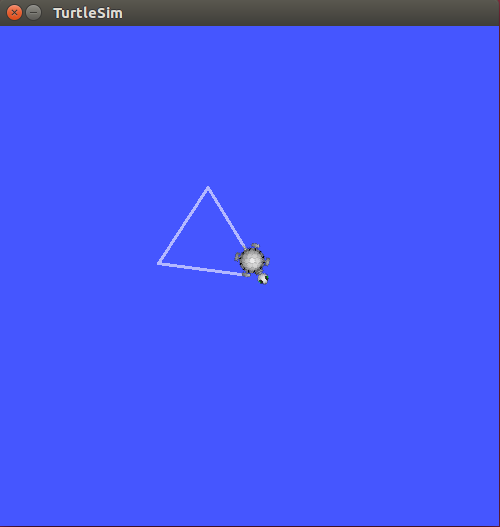
\includegraphics[scale=0.5]{image/lab2_turtlesim.png}
	\caption{\figlbl{turtle_sim} The turtlesim window}
\end{figure}

	If everything works correctly, you should see a graphical window similar to \figref{turtle_sim}.
	This window shows a simulated, turtle-shaped robot that lives in a square world.
	If you give your third terminal (the one executing the turtle\_{}teleop\_{}key command) the input focus and press the Up, Down, Left, or Right keys, the turtle will move in response to your commands, leaving a trail behind it.\\
	Making virtual turtles draw lines is not, in itself, particularly exciting.
	However, this example already has enough happening behind the scenes to illustrate many of the main ideas on which more interesting ROS systems are based.

	\item \textbf{Node} is a running instance of a ROS program. The basic command to create a node (also known as “running a ROS program”) is rosrun. ROS provides a few ways to get information about the nodes that are running
	at any particular time. To get a list of running nodes, try this command.

\begin{lstlisting}[language=bash]
# rosrun package-name executable-name
$ rosnode list
\end{lstlisting}

	If you do this in a new window, you will see a list of three nodes.

\begin{lstlisting}[language=bash]
$ /rosout
$ /turtlesim
$ /teleop_turtle
\end{lstlisting}

	The /rosout is a special node that is started automatically by roscore. Its purpose is somewhat similar to the standard output (i.e. std::cout). \\
	The other two nodes should be fairly clear: They're the simulator (turtlesim) and the teleoperation program(teleop\_{}turtle) we started ablove. \\
	You can get some information about a particular node using this command:

\begin{lstlisting}[language=bash]
$ rosnode info node-name
\end{lstlisting}

	The output includes a list of \textbf{topics} for which that node is a publisher or subscriber, the services offered by that node, its Linux process identifier
	(PID), and a summary of the connections it has made to other nodes.

	\item The primary mechanism that ROS nodes use to communicate is to send \textbf{Messages}. Messages in ROS are organized into named \textbf{Topics}.
	The idea is that a node that wants to share information will publish messages on the appropriate topic or topics;
	a node that wants to receive information will subscribe to the topic or topics that it's interested in.
	The ROS master takes care of ensuring that publishers and subscribers can find each other. \\
	This idea is probably easiest to see graphically, and the easiest way to visualize the publish-subscribe relationships between ROS nodes is to use this command:

\begin{lstlisting}[language=bash]
$ rqt_graph
\end{lstlisting}

\begin{figure}
	\centering
		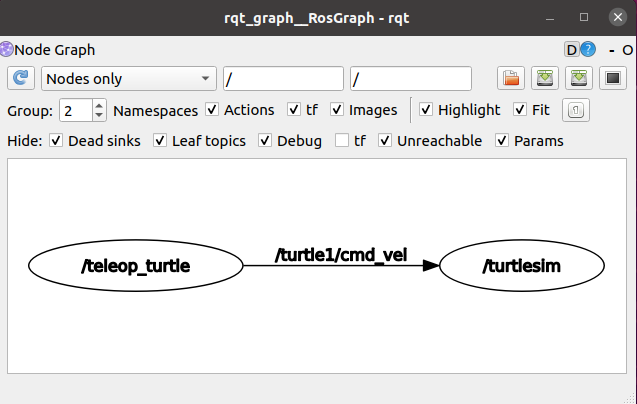
\includegraphics[scale=0.5]{image/lab2_rqt_graph.png}
	\caption{\figlbl{turtle_rqt} The rqt\_{}graph interface, showing the graph for the turtlesim example}
\end{figure}

	In this case, you will see something like \figref{turtle_rqt}. In this graph, the ovals represent nodes, and the directed edges represent publisher-subscriber relationships.
	The graph tells us that the node named /teleop\_{}turtle publishes messages on a topic called /turtle1/cmd\_{}vel, and that the node named /turtlesim subscribes to those messages. \\
	Now we can understand at least part of how the turtlesim teleoperation system works. When you press a key, the /teleop\_{}turtle node publishes messages with those movement commands on a topic called /turtle1/cmd\_{}vel. 
	Because it subscribes to that topic, the turtlesim\_{}node receives those messages, and simulates the turtle moving with the requested velocity. The important points here are:

	- The simulator doesn't care (or even know) which program publishes those cmd\_{}vel messages. Any program that publishes on that topic can control the turtle.

	- The teleoperation program doesn't care (or even know) which program subscribes to the cmd\_{}vel messages it publishes. Any program that subscribes to that topic is free to respond to those commands.
	
	\item Next let's take a closer look at the topics and messages themselves. To get a list of active topics, use this command:

\begin{lstlisting}[language=bash]
$ rostopic list
\end{lstlisting}

	In our example, this shows a list of five topics:

\begin{lstlisting}[language=bash]
$ /rosout
$ /rosout_agg
$ /turtle1/cmd_vel
$ /turtle1/color_sensor
$ /turtle1/pose
\end{lstlisting}

	You can see the autual messages that are being published on a single topic using the rostopic command, take /turtle1/pose as an exmaple:

\begin{lstlisting}[language=bash]
$ rostopic echo  /turtle1/pose
\end{lstlisting}

	your terminal will update pose data in real-time if you control the turtle by keyboard.

	Also you can learn more about a topic using the rostopic info command:

\begin{lstlisting}[language=bash]
$ rostopic info  /turtle1/pose
\end{lstlisting}

	You should see output similar to this:

\begin{lstlisting}[language=bash]
Type: turtlesim/Pose

Publishers:
  * /turtlesim (http://rvc-ece470:43601/)

Subscribers: None

\end{lstlisting}

	The most important part of this output is the very first line, which shows the \textbf{message type} of that topic. In the case of \textbf{/turtle1/pose}, the message type is 
	\textbf{turtlesim/Pose}. The message type of a topic tells you what information is included in each message on that topic, and how that information is organized.

	To see details about a message type, use a command like this:

\begin{lstlisting}[language=bash]
$ rosmsg show message-type-name
\end{lstlisting}

	Let's try using it on the message type for /turtle1/pose that we found above:

\begin{lstlisting}[language=bash]
$ rosmsg show turtlesim/Pose
\end{lstlisting}
	
	The output is:

\begin{lstlisting}[language=bash]
float32 x
float32 y
float32 theta
float32 linear_velocity
float32 angular_velocity
\end{lstlisting}

	The format is a list of fields, one per line. Each field is defined by a built-in data type (like int8, bool, or string) and a field name.
	The output above tells us that a turtlesim/Pose is a thing that contains five float32 items.

	Another example, one we'll revisit several times, is geometry\_{}msgs/Twist. This is the message type for the /turtle1/cmd\_{}vel topic, and it is slightly more complicated:

\begin{lstlisting}[language=bash]
geometry_msgs/Vector3 linear
	float64 x
	float64 y
	float64 z
geometry_msgs/Vector3 angular
	float64 x
	float64 y
	float64 z
\end{lstlisting}

	In this case, both linear and angular are \textbf{composite fields} whose date type is geometry\_{}msgs/Vector3. The indentation shows that fields named x, y, and z aremembers within
	those two top-level fields. That is, a message with type geometry\_{}msgs/Twist contains exactly six numbers, organized into two vectors called linear and angular. Each of these
	numbers has the built-in type float64.

	\item Finally, let's try to publish velocity command to the turtle in command line instead of using keyboard.
	We will use \textbf{rostopic pub} command to publish a message to a topic.

\begin{lstlisting}[language=bash]
$ rostopic pub /turtle1/cmd_vel geometry_msgs/Twist
$ "linear:
$   x: 1.0
$   y: 0.0
$   z: 0.0
$ angular:
$   x: 0.0
$   y: 0.0
$   z: -1.0" -r 1
\end{lstlisting}

	Here we are publishing a message of type geometry\_{}msgs/Twist to the topic /turtle1/cmd\_{}vel. The message is specified on the command line, and the -r option tells rostopic pub to
	publish the message repeatedly at a rate of 1 Hz. The message is specified in YAML format, which is a simple text-based format for representing structured data. The message we are
	sending is a Twist message with linear velocity 1.0 in the x direction and angular velocity -1.0 in the z direction. The turtle should move in a circle.\\
	Hint: you can utilize the full convenience of the command line by using the \textbf{tab} key to autocomplete the topic name and message type.\\

\end{enumerate}

\section{Task}

In order to master above concepts, here is one simple practice for you. We will have two turtles, as is shown in \figref{turtle_chase}. One is leader and the other is follower.
The leader turtle is controlled by keyboard input and the follower turtle should be programed to follow the trajectory.
what you should do is to write a program to make the follower turtle follow the leader turtle.\\

\begin{figure}
	\centering
		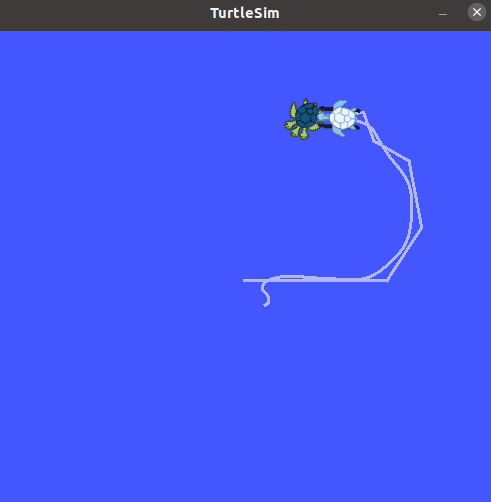
\includegraphics[scale=1]{image/lab2_turtle_chase.png}
	\caption{\figlbl{turtle_chase} turtle chase and catch game }
\end{figure}

Here give a brief introduction of the package \textbf{tf} we will use in this lab.
The \textbf{tf} package is used to keep track of multiple coordinate frames over time.

\begin{lstlisting}[language=bash]
$ roslaunch lab2pkg_turtle turtle_tf2_demo.launch
\end{lstlisting}

You will see the turtlesim start with two turtles. Once the turtlesim is started you can drive the central turtle around in the turtlesim using the keyboard arrow keys, 
select the second terminal window so that your keystrokes will be captured to drive the turtle.

This demo is using the tf2 library to create three coordinate frames: a \textbf{world} frame, a \textbf{turtle1} frame, and a \textbf{turtle2} frame.
This demo uses a tf2 broadcaster to publish the turtle coordinate frames.

\textbf{tf\_echo} reports the transform between any two frames broadcasted over ROS.

\begin{lstlisting}[language=bash]
$ rosrun tf tf_echo /world /turtle1
\end{lstlisting}

You will see the transform displayed as the \textbf{tf2\_echo} listener receives the frames broadcasted over ROS.

\begin{lstlisting}[language=bash]
At time 1622031731.625364060
- Translation: [2.796, 1.039, 0.000]
- Rotation: in Quaternion [0.000, 0.000, 0.202, 0.979]
At time 1622031732.614745114
- Translation: [1.608, 0.250, 0.000]
- Rotation: in Quaternion [0.000, 0.000, 0.032, 0.999]
\end{lstlisting}

As you drive your turtle around you will see the transform change as the two turtles move relative to each other.

Also \textbf{rviz} is a visualization tool that is useful for examining tf2 frames. 
Let's look at our turtle frames using rviz. Let's start rviz with the turtle\_rviz.rviz configuration file using the \textbf{-d} option:

\begin{lstlisting}[language=bash]
$ rosrun rviz rviz -d ${rospack find lab2pkg_turtle}/config/turtle_rviz.rviz
$ or
$ rosrun rviz rviz -d {your absolute path to turtle_rviz.rviz}
\end{lstlisting}

In the side bar you will see the frames broadcasted by tf2. As you drive the turtle around you will see the frames move in rviz.

Now you can start to write your own program to make the follower turtle follow the leader turtle.\\

\begin{figure}
	\centering
		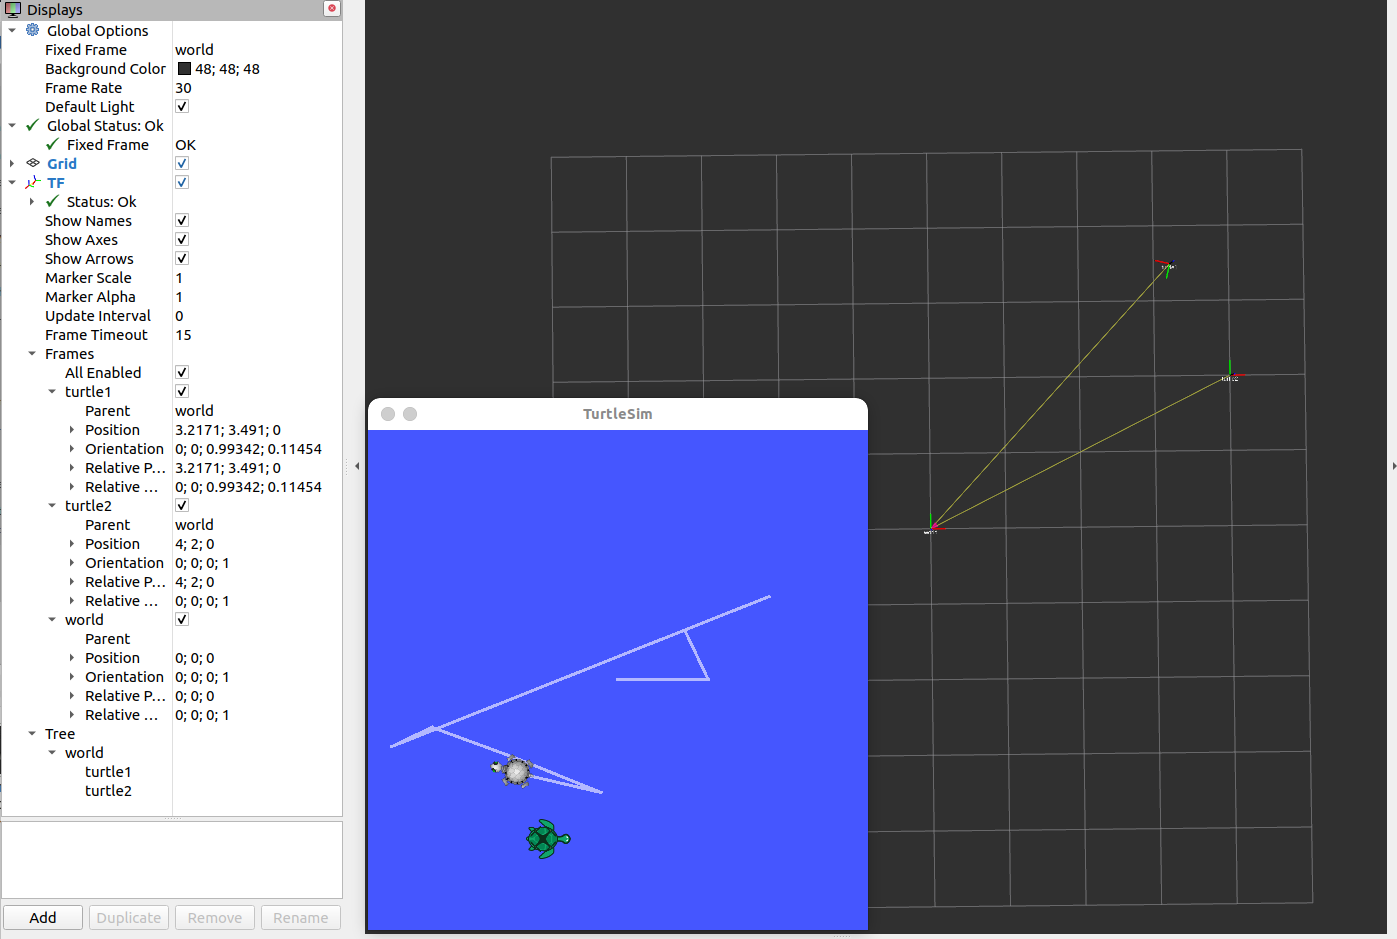
\includegraphics[scale=0.25]{image/lab2_turtle_rviz.png}
	\caption{\figlbl{turtle_rviz} The turtlesim window}
\end{figure}

\begin{enumerate}
	\item Establish your own workspace as shown in Appendix \ref{cprog} and all your programming work will be done here.
	\item Copy package \textbf{lab2pkg\_{}turtle} into your workspace. All your source code is in folder \textbf{ECE470\_LAB} on your desktop. Do Not Modify it!
	\item Complete your code and see how to run it in \textbf{README.md}.
\end{enumerate}

\section{Report}

Each partner will submit a lab report using the guidelines given in the “ECE 470: How to Write a Lab Report” document.  Please be aware of the following:
\begin{itemize}
	\item Lab reports are due one week after the final session!
	\item Lab reports will be submitted online at \href{https://learn.intl.zju.edu.cn/webapps/login/}{BlackBoard}.
\end{itemize}

\section{Demo}
Show your TA the program you created.  

\section{Grading}
\begin{itemize}
\item 10 points, completed this section by the end of the two hour lab session.  
\item 70 points, successful demonstration.
\item 20 points, report.
\end{itemize}


